\chapter{Segmentation\\ (Timothé)}

Une fois l'image pré-traitée (après la binarisation, le redressement, et la
réduction du bruit), notre algorithme de segmentation entre en jeu. Pour ce
projet d'OCR, nous avions comme objectif de traiter uniquement les cas où les
caractères sont suffisamment espacés (pas de ligature ou de lettres collées), et
où les paragraphes sont délimités par des lignes vides.

\section{Détection de lignes}

L'algorithme initial avec cette supposition est donc relativement simple et son
implémentation modulaire. La fonction prend une image en entrée, et découpe
horizontalement la prochaine ligne tant qu'aucune ligne entièrement blanche
n'est détectée. Cette partie rectangulaire de l'image est ensuite extraite, puis
passée en paramètre de la fonction de découpe des caractères.

\begin{figure}[H]
    \centering
    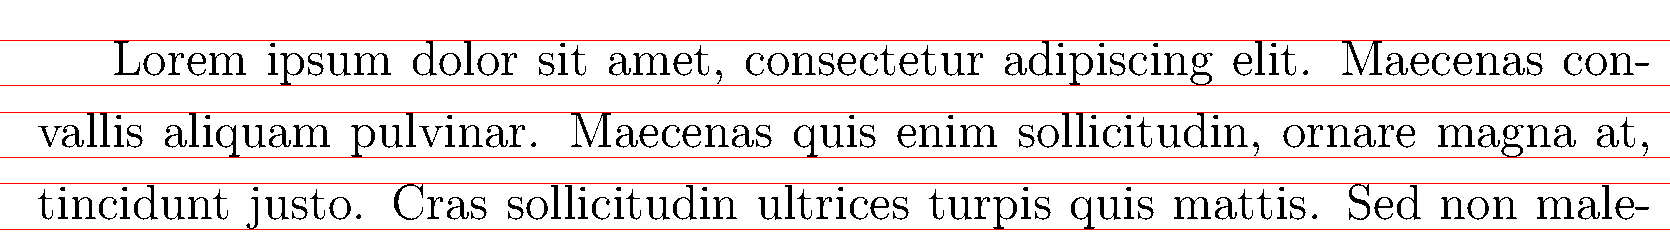
\includegraphics[width=1\textwidth]{segmentation_line}
    \caption{Segmentation des lignes}
\end{figure}

\section{Détection de caractères}

D'une manière similaire, en utilisant comme entrée une ligne de texte, la
fonction effectue une découpe verticale pour segmenter la ligne en différents
caractères.

\begin{figure}[H]
    \centering
    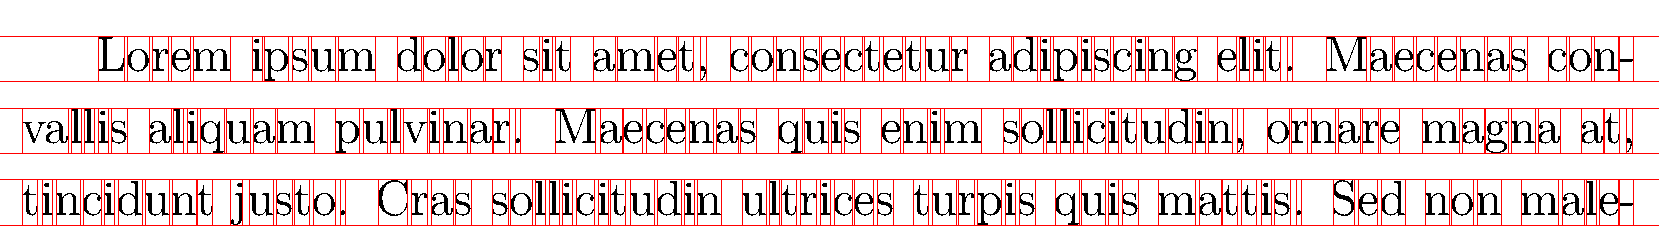
\includegraphics[width=1\textwidth]{segmentation_char}
    \caption{Segmentation des caractères}
\end{figure}

Chaque caractère extrait est ensuite redimensionné en 32x32 (pour avoir une
taille uniforme en entrée de notre réseau) à l'aide de la fonction
\mintinline{text}{SDL_BlitScaled}, puis sauvegardé au format BMP. Le réseau de
neurones pourra ainsi accéder aux caractères pré-formatés directement lors de la
reconnaissance du texte.

\section{Espacement des lignes et caractères}

Lors de la découpe, des statistiques sur les lignes et caractères sont
conservées pour plusieurs raisons. Tout d'abord cela permet d'afficher des
lignes et colonnes rouges sur l'interface graphique, indiquant visuellement la
découpe retenue (comme dans les exemples précédents). De plus, lors de la
reconstitution du texte par notre réseau, ces statistiques permettent de
déterminer où se situent les espaces et lignes vides. En effet, un simple calcul
de l'écart moyen entre des lettres permet de savoir efficacement si deux lettres
sont séparées par un espace ou non. De même, un calcul de l'espacement moyen
entre deux lignes nous permet de situer les nouveaux paragraphes.
